This section gives an application of our
theory of weak handlebodies.
We will give a classification of $2$-manifolds with finite topology.
In particular, this will imply that $\R^2$ has a unique smooth structure.

We start from the simplest case.

\begin{theorem}\label{thm:2-mfd}
Every simply connected boundaryless $2$-manifold is diffeomorphic to
either the open disk or the $2$-sphere.
\end{theorem}

\[ 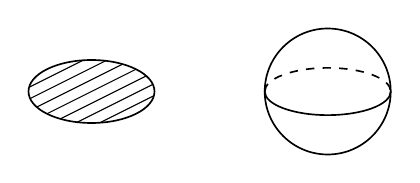
\begin{tikzpicture}[line width=.6]
    \draw (0,0) ellipse (.8 and .4);
    \begin{scope}
        \clip (0,0) ellipse (.8 and .4);
        \draw[thin] (1.7,.4) -- (.1,-.4)
                    (1.4,.4) -- (-.2,-.4)
                    (1.1,.4) -- (-.5,-.4)
                    (.8,.4) -- (-.8,-.4)
                    (.5,.4) -- (-1.1,-.4)
                    (.2,.4) -- (-1.4,-.4)
                    (-.1,.4) -- (-1.7,-.4);
    \end{scope}
    \draw (3,0) circle (.8);
    \draw[dashed] (2.2,0) arc (180:0:.8 and .3);
    \draw (2.2,0) arc (180:360:.8 and .3);
\end{tikzpicture} \]

This theorem is often proved as a consequence of
the uniformisation theorem of Riemann surfaces,
using the fact that every Riemannian $2$-manifold can be given isothermal coordinates
so that it becomes a Riemann surface.
Here we give it a new and direct proof.

\begin{proof}
By (\ref{cor:handle-decomp}) the manifold is diffeomorphic to a good $2$-handlebody $N$.
By (\ref{prop:0-handle}) we may assume it is a good weak handlebody with only one $0$-handle.
Consider the handle chain complex with $\Z_2$ coefficients
\[ \cdots\to0\to C_2(N;\Z_2)\xrightarrow{\partial_2}C_1(N;\Z_2)\xrightarrow{\partial_1}\Z_2. \]
Since $H_0(N;\Z_2)\simeq\Z_2$, we have $\partial_1=0$.
Since $N$ is simply connected, $H_1(N;\Z_2)=0$. Thus $\partial_2$ is surjective.
Note that the belt of a $1$-handle is $S^0$, i.e.\ two points.
Since $\partial_2$ is surjective,
these two points must intersect with either (a) two different $2$-handles,
or (b) only one $2$-handle in one point.
Thus we have a graph $G$,
with vertices corresponding to the $2$-handles,
and edges corresponding to $1$-handles in case (a).
For each $1$-handle in case (b), we add an ``external edge'' that connects one vertex with ``infinity''.
This can be interpreted as an infinite sequence of vertices and edges,
so that $G$ is rigorously a graph.
This graph is locally finite, and does not have \term{loops}
(i.e.\ edges whose endpoints are the same vertex).

We take a maximal tree in each connected component of $G$,
and then apply (\ref{thm-cancel-weak}) in the form of (\ref{thm:cancel-infinite}).
The effect is that these trees are collapsed.
By the same reason as above, the collapsed graph will not have loops.
Thus the resulting graph will have no edges at all.
This means that the resulting weak handlebody has no $1$-handles.
Therefore, if it has a $2$-handle, then it is the sphere;
if not, then it is the open disk.
\end{proof}

\begin{corollary}
    $\R^2$ has a unique smooth structure. \qed
\end{corollary}

This method generalises to prove the following.

\begin{theorem}\label{thm:2-mfd-noncompact}
Every connected non-compact $2$-manifold is diffeomorphic to a weak $(2,1)$-handlebody.
\end{theorem}

\begin{proof}
Similarly, the manifold is diffeomorphic to a good weak $2$-handlebody $N$
with only one $0$-handle.
We construct something like a graph, denoted $G$, in the same way,
except that edges ($1$-handles) need not have vertices ($2$-handles) as their endpoints.
We ignore those edges with no endpoints for a while,
and collapse maximal trees of connected components of the remaining part of $G$.
The resulting thing should be a collection of vertices,
each possibly with some loops attached to it,
and some isolated edges.

We need to show that there are actually no vertices.
Suppose the contrary. Then at some stage,
a first $2$-handle will be attached to a (non-weak)
$(2,1)$-handlebody with only one $0$-handle.
Since every edge is a loop, it follows that whenever the image of the attaching map
passes through a $1$-handle, it passes through both sides of it.
By an elementary argument in combinatorics, if it passes through a $1$-handle,
then it will pass through the whole boundary.
This means that there will be no boundary after this attaching,
and thus $N$ must be compact, a contradiction.
\end{proof}

Together with the following well-known result,
the preceding theorem will give a classification for
all boundaryless $2$-manifolds with finite topology.

The following result will also be proved in our handle-theoretic way.

\begin{theorem}[Classification of closed surfaces]
Every connected closed $2$-manifold is diffeomorphic to one of the following.
\begin{enum}
\item The orientable surface $\Sigma_g:=$ connected sum of $g$ tori,
where $g=0,1,\dotsc$ \emph{(where $\Sigma_0:=S^2$)}, with Euler characteristic $\chi(\Sigma_g)=2-2g$.
\item The non-orientable surface $\Pi_k:=$ connected sum of $k$ projective planes,
where $k=1,2,\dotsc$, with Euler characteristic $\chi(\Pi_k)=2-k$.
\end{enum}
\end{theorem}

\begin{proof}
Let $N$ be a good handle decomposition.
By (\ref{prop:0-handle}), we assume that $N$ has only one $0$-handle.
Taking the dual handlebody, we may assume $N$ has only one $2$-handle.
Let $k$ denote the number of $1$-handles, and we prove by induction on $k$
that the diffeomorphism type is decided by orientability and $k$.

If $k=0$, then $N\simeq S^2$. If $k=1$, an easy argument yields $N\simeq\R P^2$.
Next we suppose $k\geq2$.
If we remove the $2$-handle, we get a $(2,1)$-handlebody with boundary $S^1$.
If we remove one more $1$-handle, one of the following happens.

(i) The boundary is two circles, and the surface is orientable.
Thus the original surface is recovered by attaching a cylinder $S^1\times I$ along these circles,
and the orientability of the original surface decides how (regarding orientation) to attach this cylinder.
If we instead attach two $2$-handles along these circles,
then the Euler characteristic will increase by $2$.
By the inductive hypothesis, the resulting surface $S$ is decided by $k$.
By (\ref{prop:move-disk}) and (\ref{cor:isotopy-ext}),
if we take two disjoint disks on $S$ and remove their interiors,
then the resulting surface $S'$ is unique up to a diffeomorphism.
Thus our original surface is decided by $k$.

(ii) The boundary is two circles, and the surface is non-orientable.
This case is the same as (i) except that by (\ref{prop:move-disk}),
the two ways (regarding orientation) of attaching a cylinder result in the same surface.

(iii) The boundary is one circle.
In this case the original surface must be non-orientable,
and will be recovered by attaching a M\"obius band along the circle.
If we instead attach a $2$-handle along the circle,
then the Euler characteristic increases by $1$.
By a same argument as in (i),
it remains to show that the connected sum $\Sigma_g\mathbin\#\Pi_1$
is diffeomorphic to $\Pi_{2g}\mathbin\#\Pi_1\simeq\Pi_{2g+1}$.
This follows from the observation that $\Pi_3\simeq\Sigma_1\mathbin\#\Pi_1$.
\end{proof}

Now we may apply our results to non-compact manifolds.
We say a manifold has \term{finite topology},
if its (say $\R$-coefficient) homology groups are finite dimensional.

\begin{theorem}[Classification of $2$-manifolds]
Every connected boundaryless $2$-manifold with finite topology
is diffeomorphic to either one of the closed surfaces $\Sigma_g$ and $\Pi_k$,
or one of them with a finite number of points removed.
\end{theorem}

\begin{proof}
The compact case follows from the preceding theorem.
For the non-compact case, by (\ref{thm:2-mfd-noncompact}),
the manifold must be a weak $(2,1)$-handlebody with one $0$-handle.
By the finiteness assumption, it must have finitely many $1$-handles.
Thus it is the interior of a finite $(2,1)$-handlebody,
whose boundary is a compact $1$-manifold, i.e.\ a finite number of circles.
After attaching $2$-handles along these circles,
it would become a closed surface, whence the result follows.
\end{proof}

The remaining case to a complete classification of $2$-manifolds
is that of weak $(2,1)$-handlebodies
with one $0$-handle and infinitely many $1$-handles.
However, classifying them is very difficult,
and even the open subsets of $\R^2$ can not easily be classified.
On the other hand, we can obtain partial results.
For example, using the results in this paper, one can show that
after multiplying by $\R$,
all the orientable ones will become diffeomorphic $3$-dimensional manifolds.
